\chapter{Realtà Aumentata}

\section{Che cos’è la Realtà Aumentata?}

Per \textbf{realtà aumentata(AR, oppure Augmented Reality (RA))} \cite{augmented-reality-1}\cite{augmented-reality-2} si intende una tecnologia di computer grafica che integra in tempo reale informazioni digitali nell’ambiente reale dell’utente, arricchendone la percezione sensoriale con contenuti che i cinque sensi, da soli, non potrebbero cogliere. L’integrazione non comporta necessariamente un’aggiunta di informazioni: può consistere anche nella loro riduzione, quando ciò permette di rappresentare una situazione in modo più chiaro e utile. Gli elementi aumentati possono essere resi disponibili tramite dispositivi mobili come gli smartphone, tramite un PC dotato di webcam o di altri sensori, oppure tramite dispositivi indossabili di visione (ad es. occhiali a proiezione retinica), di ascolto (auricolari) e di manipolazione (guanti). \newline

Storicamente\cite{augmented-reality-3},le prime esperienze di realtà virtuale e aumentata risalgono agli anni ‘60. Nel 1962 Morton Heilig realizzò il Sensorama, una cabina che offriva un’esperienza multisensoriale con filmato stereoscopico, audio, vibrazioni, vento e odori, ma senza alcuna interattività. Nel 1968 Ivan Sutherland, il "padre della computer grafica", con il suo studente Bob Sproull, sviluppò il primo head-mounted display, noto come "Spada di Damocle", poichè era così pesante da dover essere sostenuto da un braccio meccanico attaccato al soffitto: mostrava grafiche wireframe tridimensionali, grazie a due tubi catodici, che seguivano i movimenti della testa, sovrapposte all’ambiente reale grazie a lenti semitrasparenti, e ne fanno quindi anche il primo sistema di AR. Il termine Augmented Reality fu coniato all’inizio degli anni '90 da Thomas Caudell e David Mizell, ricercatori della Boeing, che lo usarono per descrivere un display indossabile capace di sovrapporre al campo visivo dei tecnici le istruzioni digitali per il cablaggio degli aerei. Nel 1994 Paul Milgram e Fumio Kishino introdussero il continuum realtà-virtualità, che va dall’ambiente reale a quello completamente virtuale. Tra i due estremi si collocano l’Augmented Reality, prevalentemente reale con elementi virtuali aggiunti, e l’Augmented Virtuality, prevalentemente virtuale con elementi reali; l’intera fascia intermedia prende il nome di Mixed Reality. Infine, dalla metà degli anni 2010 si è diffuso il termine Extended Reality (XR), che non ha un singolo autore ma raggruppa VR, AR e MR.
Proprio in contemporanea all'AR, nel 1988 Mark Weiser \cite{ubiquitous-computing-1}\cite{ubiquitous-computing-2}\cite{ubiquitous-computing-3}, Chief Technologist presso il famoso centro di ricerca Xerox PARC(Palo Alto Research Center), formulò il concetto di \textbf{Ubiquitous Computing} (informatica ubiqua o pervasiva): una visione in cui i computer e le tecnologie associate diventano invisibili, fino a confondersi con la vita quotidiana. Questa invisibilità si realizza attraverso la "virtualità incarnata" (embodied virtuality), ovvero l’integrazione dei computer nel mondo fisico. Un’automobile moderna, ad esempio, può essere guidata in modo efficiente senza comprendere il funzionamento dei numerosi motori, attuatori e sensori che contiene: Weiser estese questa idea alle infrastrutture di calcolo e comunicazione, sintetizzandola così: \texttt{"Le tecnologie più profonde sono quelle che scompaiono. Si intrecciano nella trama della vita quotidiana fino a \newline diventarne indistinguibili"}\cite{ubiquitous-computing-3} \newline

L'AR si divide in due tipi\cite{The-virtuality-continuum}:
\begin{itemize}
    \item \textbf{Spatial AR}, Proietta la luce direttamente sull'ambiente reale (usando video proiettori fisici fissati nella stanza). Non richiede visori o smartphone per essere vista. Un esempio tipico è il spatial projection mapping (es. proiettare la trama di un tessuto su un divano reale). Consiste proprio nel proiettare interfacce o elementi digitali su superfici reali (tavoli, pareti, oggetti) e rendere quelle superfici interattive.

     \begin{figure}[H]
            \centering
            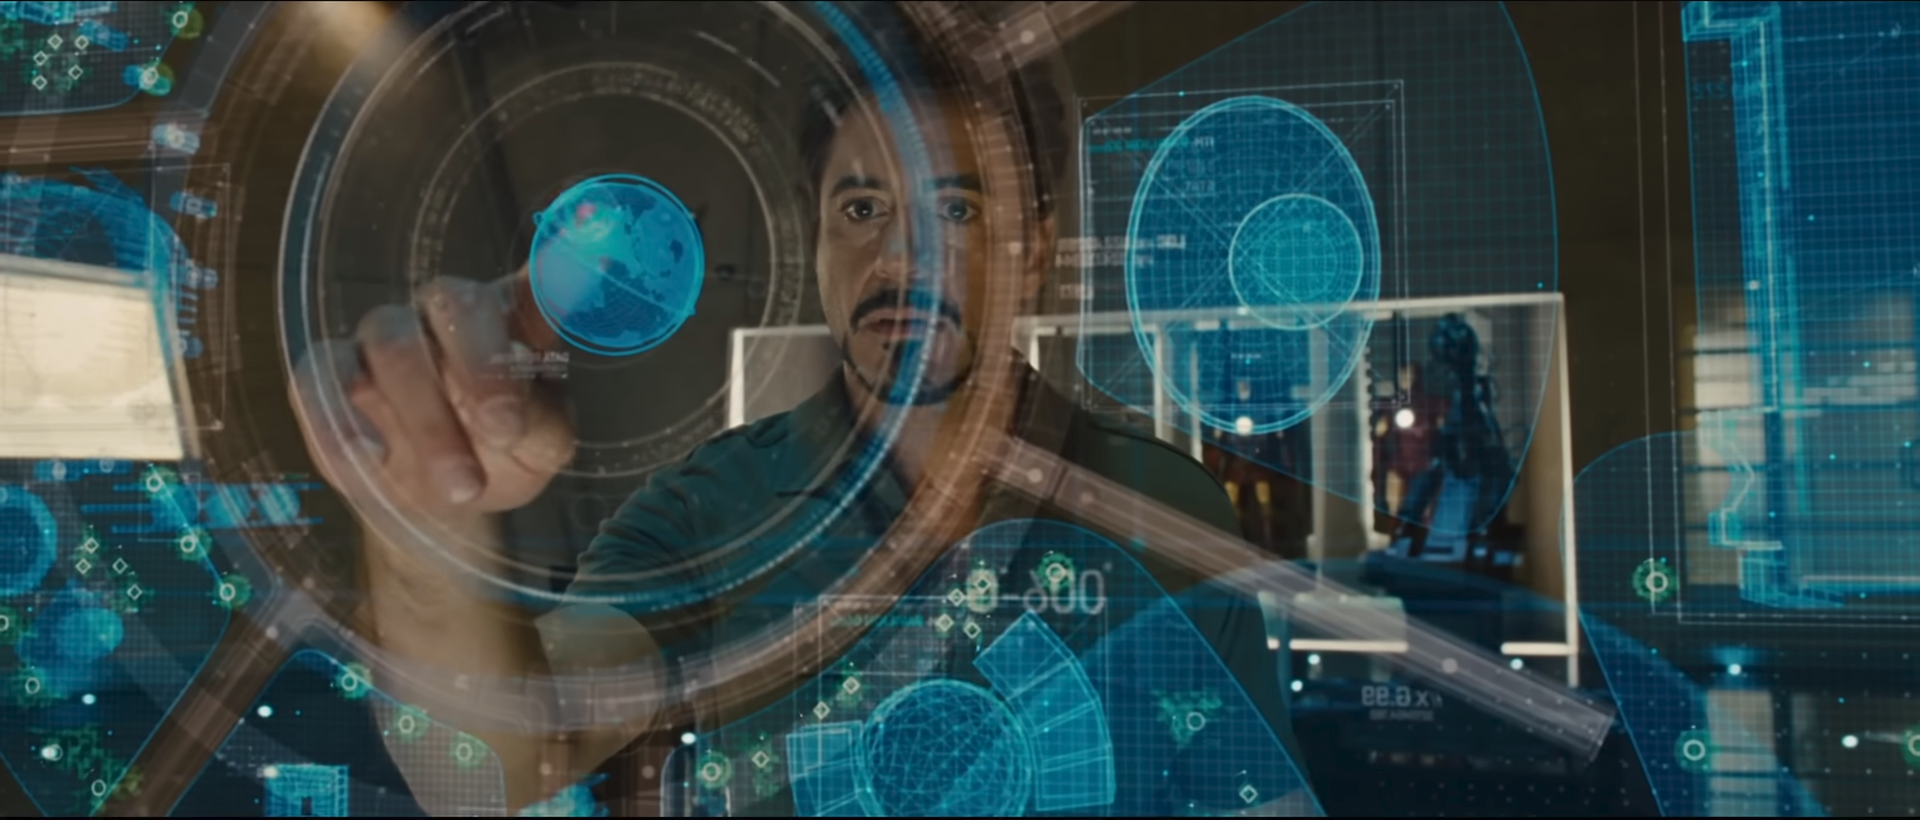
\includegraphics[width=0.7\textwidth]{images/augmented-reality/Spatial-AR.png} 
            \caption{Scene of Iron Man 2 (2010)\cite{img-ironman}}
            \label{fig:dt}
    \end{figure}

    
     \item \textbf{See-through AR}, in cui si fa uso di periferiche o dispositivi indossabili o di semplice visualizzazione come visore o schermi.

     \begin{itemize}
         \item \textbf{Optical See-through}, Vetri o lenti trasparenti (come i Google Glass o i Magic Leap) in cui la luce reale passa direttamente e le immagini digitali vengono proiettate sopra, quindi vedi il mondo reale direttamente con i tuoi occhi e la grafica vi viene sovrapposta tramite prismi/specchi.

        \begin{figure}[H]
            \centering
            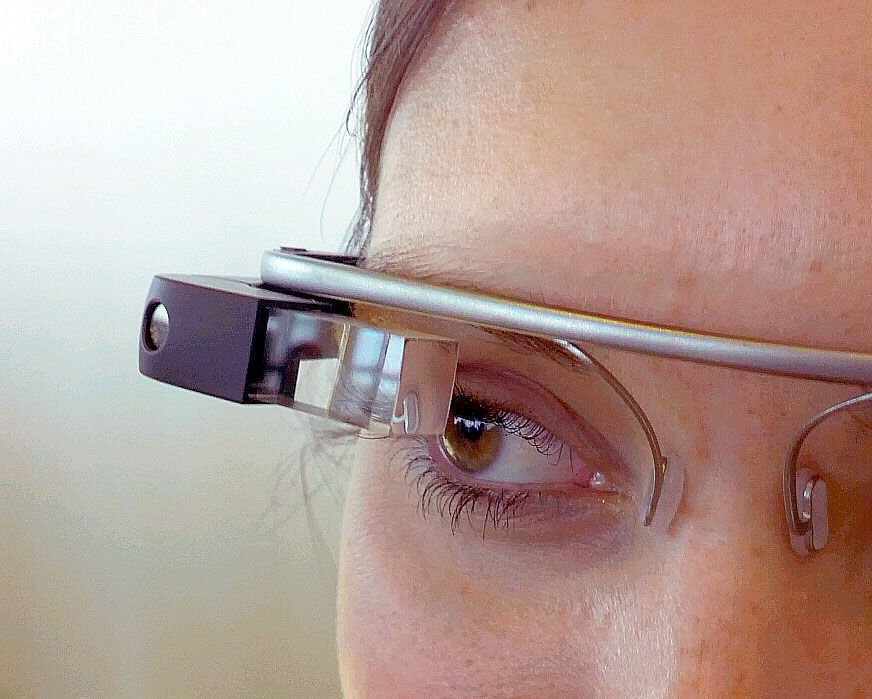
\includegraphics[width=0.6\textwidth]{images/augmented-reality/Google_Glass_detail.jpg} 
            \caption{Google Glass, 2013 \cite{img-google_glass}}
            \label{fig:dt}
        \end{figure}

         
         \item \textbf{Video See-through (Passthrough)}, che catturano il mondo reale tramite telecamere e lo riproiettano su schermi interni ad altissima risoluzione insieme agli elementi digitali. Visori chiusi (es. Apple Vision Pro, Meta Quest 3) o dispositivo con camera (es. Invizimals su PSP), dove microcamere riprendono l'esterno e mostrano il video su uno schermo insieme alla grafica 3D.

        \begin{figure}[H]
            \centering
            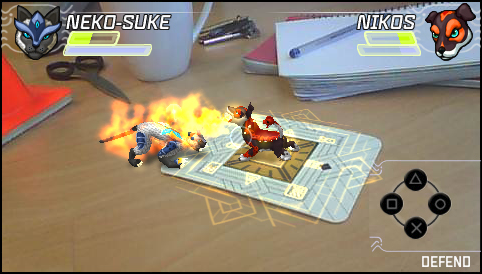
\includegraphics[width=0.7\textwidth]{images/augmented-reality/invizimals.png} 
            \caption{An example of AR videogame: Invizimals, game of PSP \cite{img-invizimals}}
            \label{fig:dt}
        \end{figure}
     \end{itemize}

\end{itemize}


Dalla definizione precedentemente scritta, si può dedurre che l'AR è adatta ad ogni ambito\cite{augmented-reality-1}: 

\begin{itemize}
    \item[-] \textbf{ Medicina e Sanità} \newline
    in medicina e sanità si introduce per migliorare la chirurgia assistita, ovvero tramite sovrapposizione di scansioni (TAC, risonanze) direttamente sul corpo del paziente durante gli interventi per guidare l'incisione e la precisione del chirurgo, e sempre in questo ambito, si usa per la formazione di medici mediante simulazioni delle procedure mediche e anatomiche su modelli virtuali interattivi senza rischi per i pazienti;

     \item[-] \textbf{ Industria e Luogo Lavorativo} \newline
    nell'industria e in ambito lavorativo in generale viene introdotta nella manutenzione e assemblaggio, mediante istruzioni di montaggio o schemi tecnici sovrapposti in tempo reale sui macchinari per guidare i tecnici a mani libere (remote assistance), e anche sulla sicurezza, in cui consiste nella segnalazione visiva di pericoli o aree ad alto rischio direttamente nel campo visivo degli operatori;

     \item[-] \textbf{ Architettura, Progettazione e Pianificazione Urbana} \newline
    in architettura, progettazione e pianificazione Urbana viene usata nella visualizzazione dei progetti, per il rendering 3D di edifici o strutture sovrapposti sul terreno reale prima dell'inizio dei lavori, oppure per l'ispezione di interni, offrendo la possibilità di guardare "attraverso le pareti" per individuare tubature, cablaggi o elementi strutturali interni;

     \item[-] \textbf{ Archeologia, Cultura e Turismo} \newline
    In archeologia, cultura e turismo viene impiegato nella ricostruzione di rovine, nella visualizzazione in tempo reale di come apparivano monumenti ed edifici antichi direttamente sopra i siti archeologici attuali, e nelle guide ed esperienze di musei, tramite punti di interesse interattivi e contenuti multimediali sovrapposti alle opere o alle attrazioni turistiche della città;

     \item[-] \textbf{Commercio, Marketing e Retail} \newline
    nel commercio, marketing e retail, con la famosa filosofia del "Try Before You Buy" (Prova prima di acquistare): con la visualizzazione di mobili e oggetti d'arredo nell'ambiente di casa prima dell'acquisto, oppure prova virtuale di capi d'abbigliamento, occhiali e cosmetici, e con l'Augmented Advertising, che consiste in campagne pubblicitarie interattive accessibili inquadrando imballaggi, riviste o cartelloni;

     \item[-] \textbf{ Istruzione e Formazione (STEM)} \newline
    nell'istruzione e formazione (STEM) tramite libri e materiali interattivi, ovvero con l'integrazione dei libri di testo classici con modelli 3D animati di molecole, organi o corpi celesti e in ambito più pratico con l'addestramento al volo e militare tramite display o visori per piloti (Head-Up Display o HUD) con dati tattici, rotte e parametri di volo sovrapposti al parabrezza;

     \item[-] \textbf{Automotive e Navigazione} \newline
    nell'automotive e navigazione sempre usando l'implementazione precedente, ovvero tramite Head-Up Display (HUD) proiettando i dati di navigazione, velocità e segnali stradali direttamente sul parabrezza dell'auto, e nella navigazione pedonale o per veicoli, tramite indicazioni stradali visive e frecce dinamiche sovrapposte direttamente sulla strada inquadrata dalla fotocamera;
     
     \item[-] \textbf{ Intrattenimento e Videogiochi} \newline
    nell'intrattenimento e nei videogiochi, in cui consiste nel gaming geolocalizzato, ovvero videogiochi che trasformano l'ambiente cittadino reale in un campo da gioco interattivo (es. Pokemon GO);

     \item[-] \textbf{ Eventi dal Vivo e Trasmissioni} \newline
    infine negli eventi dal vivo e trasmissioni, mediante grafiche e statistiche in tempo reale sovrapposte ai campi durante gli eventi sportivi.
\end{itemize}

\section{ Pro e Contro }
In tutti questi ambiti, possiamo studiare e analizzare come l'AR si comporta sotto diversi aspetti e stilare una lista di caratteristiche che può portare questa tecnologia, sia positive sia negative.

\subsection{Pro}

\begin{enumerate}
    \item \textbf{Continuità con la realtà e sicurezza d'uso} \newline
    A differenza della realtà virtuale (VR), che isola completamente l'utente portandolo in un mondo artificiale, la realtà aumentata mantiene la persona ancorata all'ambiente fisico reale. Questo offre vantaggi cruciali:
    \begin{itemize}
        \item \textbf{Consapevolezza dell'ambiente circostante} \newline
        L'utente continua a vedere dove cammina o lavora, riducendo rischi di collisione o disorientamento.
        \item \textbf{Minore affaticamento visivo/sensoriale} \newline
        Non dovendo ricreare un intero mondo 3D ma solo "strati" di informazione, l'esperienza risulta spesso più naturale e meno alienante.
    \end{itemize}

    \item \textbf{Miglioramento della precisione e riduzione degli errori umani} \newline
    La sovrapposizione visiva di dati e modelli direttamente sull'oggetto o sul corpo su cui si sta lavorando elimina la necessità di consultare continuamente manuali o schermi esterni:
    \begin{itemize}
        \item \textbf{Minori tassi di errore} \newline
        In ambiti critici come la chirurgia o la manutenzione industriale, le guide visive passo-passo riducono le dimenticanze e gli sbagli operativi.
        \item \textbf{Aumento della velocità di esecuzione} \newline
        L'operatore o il tecnico ha le mani libere e le informazioni visive posizionate esattamente dove servono.
    \end{itemize}

    \item \textbf{Abbattimento dei costi e ottimizzazione dei processi} \newline
    \begin{itemize}
        \item \textbf{Prototipazione e visualizzazione anticipata} \newline
        Architetti, designer e pianificatori possono testare un progetto nell'ambiente reale prima di costruire o produrre fisicamente il bene, riducendo lo spreco di materiali e correggendo difetti in anticipo.
        \item \textbf{Riduzione dei resi nel commercio} \newline
        La possibilità di provare virtualmente mobili o vestiti prima dell'acquisto ("Try Before You Buy") aumenta la certezza del consumatore e abbassa la quota di resi.
    \end{itemize}

    \item \textbf{Esperienza di apprendimento più intuitiva e coinvolgente} \newline
    \begin{itemize}
        \item \textbf{Apprendimento con l'esperienza} \newline
        Sia nell'istruzione scolastica (STEM) sia nella formazione aziendale, visualizzare ed interagire con oggetti 3D (come molecole, motori o organi anatomici) facilita la comprensione di concetti complessi rispetto alla sola lettura.
        \item \textbf{Accessibilità del sapere} \newline
        Le informazioni guida o storiche vengono erogate in modo contestuale (es. inquadrando un monumento o una rovina), rendendo l'esplorazione autonoma e ricca di valore culturale.
    \end{itemize}

    \item \textbf{Collaborazione e assistenza a distanza} \newline
    \begin{itemize}
        \item \textbf{Remote Assistance} \newline
        Esperti qualificati possono guidare tecnici o utenti sul campo disegnano indicazioni visive direttamente nello schermo di chi opera, eliminando tempi e costi di trasferta.
        \item \textbf{Lavoro di squadra facilitato} \newline
        Più persone possono visualizzare e manipolare simultaneamente lo stesso modello 3D nello spazio reale.
    \end{itemize}

\end{enumerate}


\subsection{Contro}

Nonostante i numerosi vantaggi, la diffusione della realtà aumentata comporta diversi rischi, pericoli e svantaggi che spaziano dalla sicurezza fisica alle implicazioni etiche e sociali.

\begin{enumerate}
    \item \textbf{Rischi per la sicurezza fisica e distrazione} \newline
    \begin{itemize}
        \item \textbf{Saturazione cognitiva e perdita di attenzione} \newline
        L'accumulo di informazioni visive sovrapposte al mondo reale può sovraccaricare il cervello, riducendo la prontezza di riflessi in situazioni critiche (come la guida di veicoli o la gestione di macchinari)
        \item \textbf{Incidenti da distrazione} \newline
        L'uso continuo di visori o smartphone per interagire con contenuti AR nell'ambiente urbano aumenta il rischio di cadute, attraversamenti involontari o collisioni con ostacoli e persone.
    \end{itemize}

     \item \textbf{Privacy e sorveglianza invasiva} \newline
    \begin{itemize}
        \item \textbf{Raccolta costante di dati ambientali e personali} \newline
        Per funzionare, i dispositivi AR utilizzano fotocamere e sensori sempre attivi che mappano continuamente l'ambiente circostante, registrando volti di passanti, targhe ed spazi privati senza consenso esplicito.
        \item \textbf{Tracciamento dei comportamenti e biometria} \newline
        I visori avanzati monitorano lo sguardo (eye tracking), i movimenti del corpo e le reazioni emotive, fornendo alle aziende dati estremamente sensibili sulle preferenze e sull'attenzione degli utenti.

    \end{itemize}

    \item \textbf{Sicurezza informatica e manipolazione della realtà} \newline
    \begin{itemize}
        \item \textbf{Hacking ed estorsione informativa} \newline
        Un attacco informatico potrebbe iniettare informazioni false nel campo visivo dell'utente (ad esempio alterare i segnali stradali su un display guida o nascondere un ostacolo reale), con conseguenze potenzialmente fatali, portando quindi a danni irreversibili o comunque molto gravi ad ambiente, beni o addirittura persone.

        \item \textbf{Falsificazione del contesto (Reality Hacking)} \newline
       Sovrapporre elementi grafici non autorizzati o ingannevoli su luoghi fisici (come pubblicità abusive, messaggi diffamatori o informazioni manipolate) può alterare la percezione della realtà da parte degli utenti.

    \end{itemize}

     \item \textbf{Impatto Psicologico e Dipendenza} \newline
     Rischi in comune con i Social Network:
    \begin{itemize}
        \item \textbf{Sovraccarico sensoriale e alienazione} \newline
        La costante sovrapposizione di notifiche e contenuti digitali al mondo fisico rende difficile la disconnessione, aumentando i livelli di stress e ansia.

        \item \textbf{} Un utilizzo incontrollato può portare a preferire l'ambiente arricchito dai filtri digitali rispetto al mondo reale, condizionando negativamente la socializzazione e le relazioni interpersonali dirette.


    \end{itemize}

    \item \textbf{Limiti Tecnici ed Economici} \newline
     
    \begin{itemize}
        \item \textbf{Costi elevati dei dispositivi} \newline
        I visori e gli strumenti AR di livello professionale mantengono prezzi accessibili solo a grandi aziende o settori specializzati, rischiando di ampliare il divario digitale (digital divide)

        \item \textbf{Consumo energetico e limiti hardware} \newline
        I sensori e i processori AR richiedono un'elevata potenza di calcolo, comportando una durata limitata della batteria e problemi di surriscaldamento nei dispositivi portatili.


    \end{itemize}

\end{enumerate}



\section{ Come funziona? }

\textbf{Architettura}
 \begin{figure}[H]
            \centering
            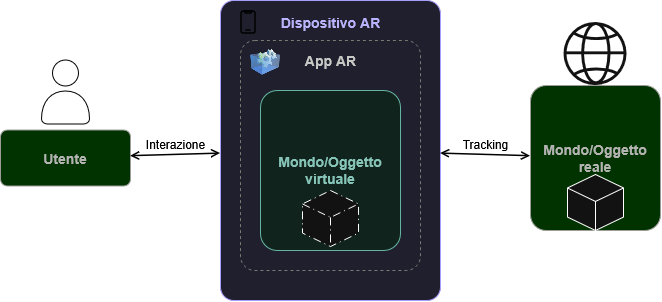
\includegraphics[width=0.8\textwidth]{images/augmented-reality/AR-Working-General-Architecture.png} 
            \caption{AR General Working Architecture\cite{img-ar-architecture}}
            \label{fig:dt}
\end{figure}

Il funzionamento di un sistema di AR si basa su un ciclo continuo di elaborazione (loop di feedback) suddiviso in tre fasi sequenziali fondamentali\cite{augmented-reality-2}:

\begin{figure}[H]
            \centering
            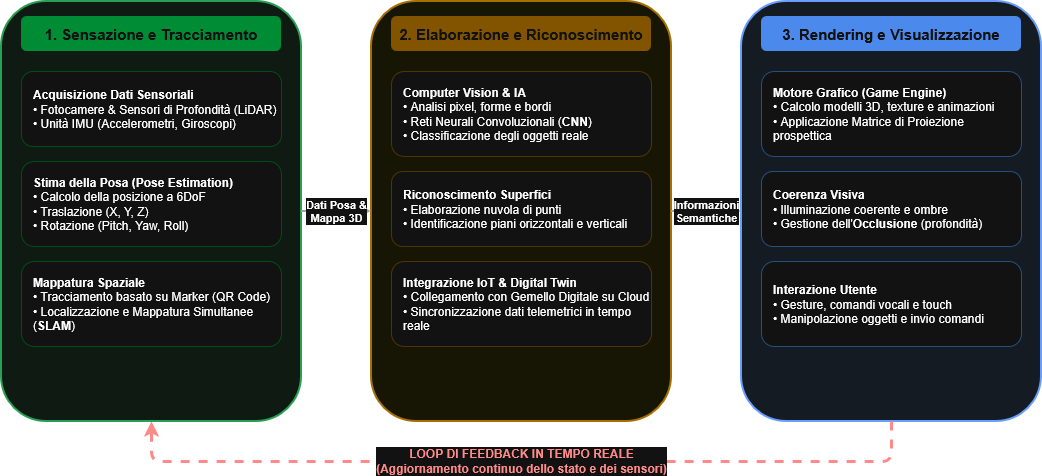
\includegraphics[width=1\textwidth]{images/augmented-reality/The-typical-pipeline-of-an-AR-application.png} 
            \caption{AR Pipeline}
            \label{fig:dt}
    \end{figure}

\begin{itemize}
    \item \textbf{Sensazione e Tracciamento} \newline
    Per fare in modo che gli elementi virtuali possano essere inseriti nel mondo reale in modo credibile, uno smartphone o un visore devono comprendere in tempo reale e con estrema precisione dove si trovano nello spazio tridimensionale. Per ottenere questo risultato, il dispositivo si affida all'acquisizione continua di flussi video e dati fisici attraverso una combinazione di sensori ottici e inerziali. Tra i sensori ottici troviamo le fotocamere tradizionali, che riprendono l'ambiente circostante, e i sensori di profondità avanzati come il LiDAR, che emettono impulsi di luce invisibile per calcolare la distanza esatta degli oggetti e creare una mappa tridimensionale millimetrica dello spazio. A questi si affiancano l'Unità di Misura Inerziale, comunemente nota come IMU, che integra accelerometri per misurare le variazioni di velocità e giroscopi per tracciare l'orientamento e la velocità di rotazione. Grazie a questa componentistica, il sistema è in grado di captare anche i movimenti minimi o rapidi della testa o delle mani dell'utente, compensando i ritardi visivi e garantendo la fluidità dell'esperienza. \newline

    L'aspetto più importante di questa fase è la cosiddetta stima della posa, o Pose Estimation, che calcola la posizione e l'orientamento del dispositivo in sei gradi di libertà, noti come 6DoF. Questi sei gradi descrivono tutte le possibili modalità di movimento di un corpo nello spazio: tre riguardano la traslazione lineare lungo gli assi cartesiani, ovvero lo spostamento in avanti e indietro, a sinistra e a destra, e in alto e basso; gli altri tre riguardano la rotazione, specificatamente l'inclinazione in avanti e indietro nota come pitch, la rotazione orizzontale a destra e sinistra nota come yaw, e l'inclinazione laterale nota come roll. Per calcolare questi dati e mappare l'ambiente, i dispositivi utilizzano principalmente due strade. La prima è il tracciamento basato su marcatori, o Marker-based, in cui il software riconosce simboli o pattern geometrici prestampati, come i codici QR; conoscendo le dimensioni e la posizione esatta del marcatore nel mondo reale, il sistema sa immediatamente dove posizionare il contenuto virtuale. La seconda tecnica, molto più avanzata e utilizzata negli ambienti aperti o non preparati, è la localizzazione e mappatura simultanee, nota come SLAM. Questa tecnologia consente al dispositivo di costruire progressivamente una mappa 3D dell'ambiente circostante e, nello stesso identico momento, di calcolare la propria posizione esatta all'interno di quella mappa senza bisogno di alcun punto di riferimento esterno, permettendo all'utente di muoversi liberamente.

    \begin{figure}[H]
            \centering
            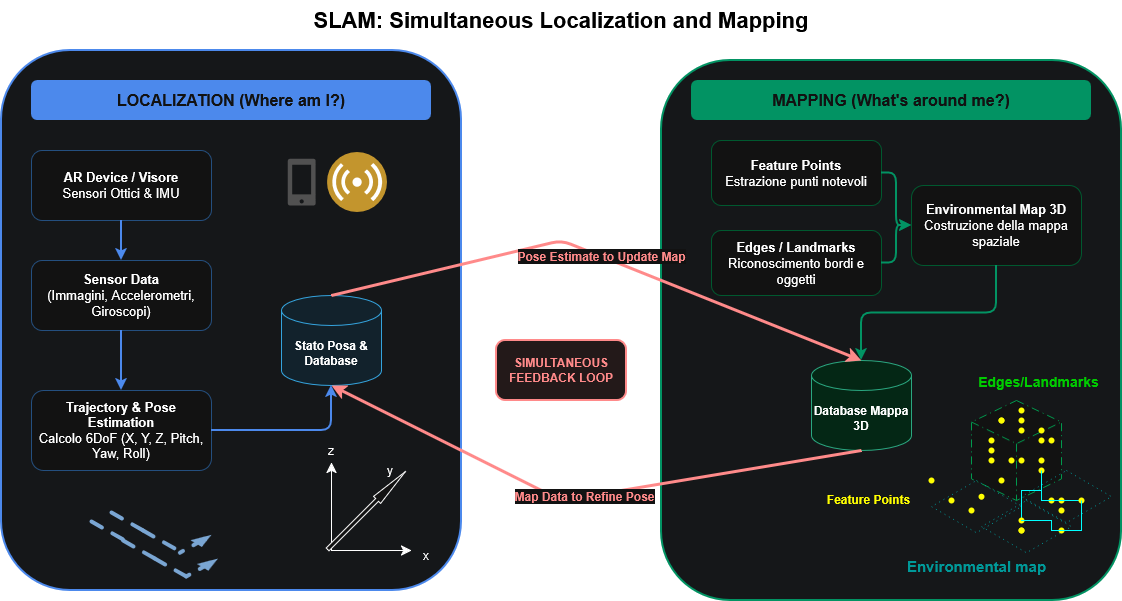
\includegraphics[width=1\textwidth]{images/augmented-reality/SLAM.png} 
            \caption{SLAM \cite{img-SLAM}}
            \label{fig:dt}
    \end{figure}

    \item \textbf{Elaborazione e Riconoscimento} \newline
    Una volta che i dati grezzi sono stati raccolti dai sensori e dalle fotocamere, il software li interpreta e cerca di dare un significato logico e semantico a ciò che la telecamera sta inquadrando. Questo processo si fonda sui principi della Computer Vision, ovvero la branca dell'intelligenza artificiale che permette ai computer di "vedere" e comprendere le immagini e i video digitali, analizzando i singoli pixel per riconoscere bordi, forme, angoli e variazioni di luce. Per fare un salto di qualità nell'interpretazione dell'ambiente, gli algoritmi si affidano a modelli di intelligenza artificiale complessi, come le reti neurali convoluzionali, note anche come CNN. Queste reti di apprendimento profondo sono particolarmente abili nell'elaborazione visiva e consentono al sistema di classificare gli oggetti con precisione, distinguendo ad esempio un tavolo da una sedia, una parete da una porta, oppure riconoscendo un componente meccanico specifico all'interno di un'officina.    \newline

    Attraverso questo processo, il software riesce a riconoscere i piani e le superfici fisiche presenti nell'ambiente, elaborando la nuvola di punti creata nella fase precedente per identificare le superfici orizzontali, come pavimenti e tavoli, e quelle verticali, come le pareti. Questa capacità è fondamentale perché permette agli oggetti virtuali di "posarsi" in modo logico sul mondo reale, come fare in modo che una sedia olografica poggi saldamente sul pavimento di una stanza. In contesti industriali o smart factories particolarmente avanzati, questa fase di riconoscimento si spinge oltre, prevedendo l'interconnessione con un Digital Twin, ovvero un gemello digitale memorizzato sul cloud. Quando il sistema inquadra un macchinario reale, non si limita a riconoscerne la forma geometrica nello spazio, ma lo associa alla sua controparte virtuale dinamica. Questo collegamento permette di sincronizzare in tempo reale i dati telemetrici, come la pressione, la temperatura e i cicli di lavoro, e lo stato di salute dell'impianto provenienti dai sensori IoT, ovvero gli oggetti intelligenti connessi a Internet, consentendo all'operatore di visualizzare grafici, schemi e avvisi diagnostici direttamente sovrapposti al macchinario che sta guardando.

    \item \textbf{Rendering e Visualizzazione} \newline
    Infine il software si occupa di generare concretamente l'immagine finale che l'utente vedrà attraverso lo schermo del dispositivo, fondendo in modo fluido, coerente e in tempo reale il mondo reale con quello virtuale. A occuparsi di questo compito è il motore grafico, o Game Engine, un software potente originariamente sviluppato per l'industria dei videogiochi ma oggi indispensabile in AR, che si incarica di calcolare la geometria dei modelli tridimensionali, applicare le texture, cioè i materiali visivi e i colori, gestire le animazioni e simulare le leggi della fisica sugli oggetti olografici. Per fare in modo che l'illusione ottica sia perfetta, il motore grafico applica una matrice di proiezione, ovvero un calcolo matematico basato sulla posizione esatta del visore rilevata nella prima fase di tracciamento. Questo calcolo deforma e scala gli oggetti 3D rispettando le regole della prospettiva umana, facendo in modo che gli elementi virtuali vicini appaiano più grandi e quelli lontani più piccoli. \newline

    La coerenza visiva viene mantenuta grazie a due elementi cruciali: l'illuminazione coerente e l'occlusione. Nel primo caso, il sistema analizza le fonti di luce presenti nell'ambiente reale e illumina di conseguenza l'oggetto virtuale, generando ombre realistiche che ne impediscono l'effetto "piatto" o posticcio. Nel secondo caso, l'occlusione risolve il problema della profondità gestendo le sovrapposizioni: se una persona passa la mano o un oggetto reale davanti a un ologramma, la mano deve coprire l'oggetto virtuale perché si trova più vicina agli occhi rispetto ad esso. Senza l'occlusione, l'ologramma rimarrebbe sempre visibile in primo piano, rovinando completamente il senso di immersione. Infine, il ciclo si completa gestendo l'interazione dell'utente: attraverso gesture, ossia i movimenti delle mani tracciati dalle telecamere, comandi vocali o input touch, l'utente può manipolare l'oggetto virtuale, spostandolo, ridimensionandolo o aprendolo, oppure può inviare comandi diretti che modificano lo stato del mondo reale o dei sistemi fisici connessi.


\end{itemize}


\section{Tipologie di Realtà Aumentata}
Ne esistono due tipi: AR a riconoscimento Marker,la quale è più economica e accessibile, e Markerless AR, la quale offre un coinvolgimento maggiore.

\subsection{AR a Riconoscimento Marker}
Con questa tipologia, affinchè avvenga l'implementazione dell'AR, è necessario un trigger fisico (Marker) nell'ambiente reale, ad esempio un codice QR, un'immagine o un altro marker di destinazione. Quando la fotocamera di un dispositivo rileva il marker, attiva la visualizzazione dell'esperienza AR associata. Poiché questo tipo di AR è accessibile in qualsiasi momento da una serie di dispositivi, è quello più flessibile.
\subsection{Markerless AR}
Con questa tipologia, invece, non c'è alcun bisogno di un trigger fisico, poichè si basa direttamente su sensori, GPS, accelerometri e fotocamere del dispositivo per mappare in tempo reale l'ambiente circostante dell'utente. Questo mapping avviene spesso grazie ad algoritmi e alla computer vision, i quali determinano dove posizionare i contenuti digitali, rendendo l'esperienza più spontanea e dinamica.
 
\section{AR vs VR vs XR vs MR vs Spatial Computing}
Ora vedremo la differenza tra queste tecnologie molto simili ma diverse tra loro\cite{ar-vs-other}\cite{The-virtuality-continuum}:

\begin{itemize}
    \item \textbf{Virtual Reality (VR)} \newline
    Permette la creazione e l'immersione in un ambiente virtuale 3D, consentendo all'utente di muoversi liberamente e di interagire con esso. È possibile grazie ad elaboratori e interfacce dedicate, come visori, guanti dati (\textit{wired gloves}), cybertute e piattaforme omnidirezionali. Viene utilizzata per simulazioni, videogiochi e addestramento; un esempio diffuso è la serie di visori Meta Quest.
    Esistono due tipi: 
    \begin{itemize}
        \item \textbf{Semi-Immersive VR}, nel quale i dispositivi VR rappresentano in modo preciso e reale una parte del punto di vista dell'utente
         \item \textbf{Immersive VR}, dove i dispositivi rappresentano l'intero punto di vista dell'utente. 
    \end{itemize}

    \item \textbf{Spatial Computing} \newline
    È il paradigma tecnologico che consente ai sistemi informatici di comprendere, mappare e interagire con lo spazio fisico 3D così come fanno gli esseri umani. Permette ai contenuti digitali di "vivere" nell'ambiente reale con persistenza spaziale (ad esempio, posizionare un quadro digitale su una parete reale e ritrovarlo esattamente nella stessa posizione al successivo utilizzo del visore). Lo Spatial Computing fornisce le basi tecnologiche necessarie per abilitare la Mixed Reality.
    
    \item \textbf{Mixed Reality (MR)} \newline
    Fonde il mondo fisico e gli oggetti digitali, permettendo un'interazione dinamica in tempo reale tra elementi reali e virtuali (ad esempio, una palla virtuale che rimbalza sul pavimento reale di una stanza), che sfrutta lo Spatial Computing. Un esempio di dispositivo MR avanzato è l'Apple Vision Pro.

    \begin{figure}[H]
        \centering
        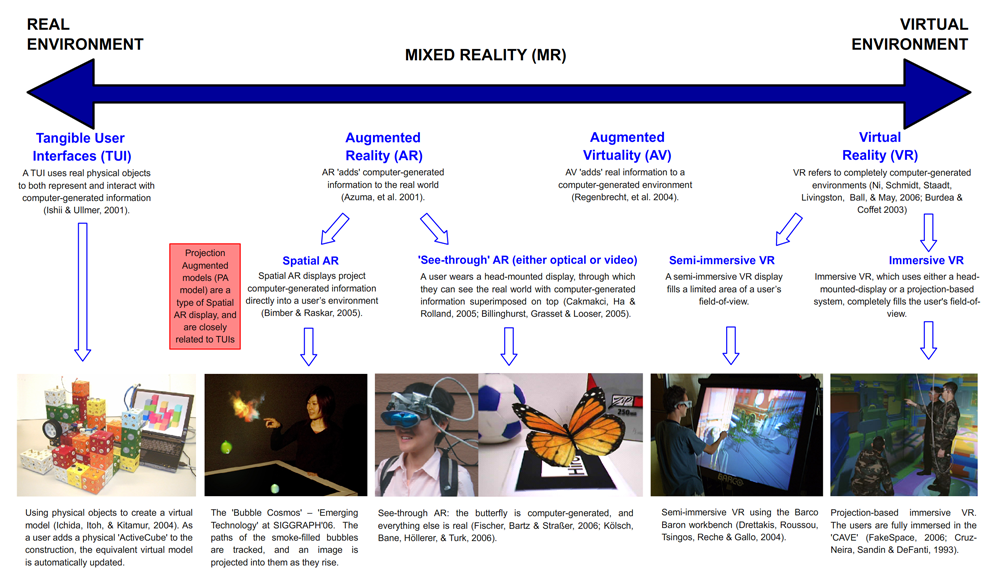
\includegraphics[width=0.7\textwidth]{images/augmented-reality/MR.png} 
        \caption{The Reality-Virtuality Continuum according to Milgram \cite{The-virtuality-continuum}}
        \label{fig:dt}
    \end{figure}

     dove AV è Augmented Virtuality, una tecnologia di MR in cui l'ambiente generato al computer viene arricchito da oggetti del mondo fisico. 
    
    \item \textbf{Extended Reality (XR)} \newline
    Termine che racchiude VR, AR e MR. Quando un dispositivo viene definito XR (come Apple Vision Pro o Galaxy XR), significa che è in grado di passare fluidamente tra diverse modalità di realtà immersiva. 
    
    In questo ambito rientra anche la \textbf{Augmented Reality (AR)} come detto in precedenza: l'integrazione in tempo reale di informazioni digitali nell'ambiente reale dell'utente, percepibili tramite dispositivi come smartphone, visori o auricolari. Tale integrazione può operare sia per addizione di elementi multimediali, sia per sottrazione di informazioni superflue (diminuzione della realtà), al fine di rendere la percezione dell'ambiente più chiara e funzionale.
    
\end{itemize}


